\documentclass{standalone}
\usepackage{tikz}
\begin{document}
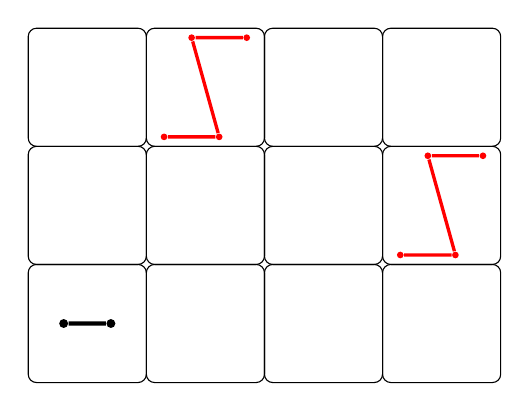
\begin{tikzpicture}[scale=1.5]
  % draw rounded cell boxes
  \draw[rounded corners=3pt] (0,0) rectangle (1,1);
  \draw[rounded corners=3pt] (0,1) rectangle (1,2);
  \draw[rounded corners=3pt] (0,2) rectangle (1,3);
  \draw[rounded corners=3pt] (1,0) rectangle (2,1);
  \draw[rounded corners=3pt] (1,1) rectangle (2,2);
  \draw[rounded corners=3pt] (1,2) rectangle (2,3);
  \draw[rounded corners=3pt] (2,0) rectangle (3,1);
  \draw[rounded corners=3pt] (2,1) rectangle (3,2);
  \draw[rounded corners=3pt] (2,2) rectangle (3,3);
  \draw[rounded corners=3pt] (3,0) rectangle (4,1);
  \draw[rounded corners=3pt] (3,1) rectangle (4,2);
  \draw[rounded corners=3pt] (3,2) rectangle (4,3);
  % draw black chords for chord_row_cells
  \node[circle, fill=black, inner sep=0.04cm] (chord_row0_left) at (0.3,0.5) {};
  \node[circle, fill=black, inner sep=0.04cm] (chord_row0_right) at (0.7,0.5) {};
  \draw[black, line width=1.5pt] (chord_row0_left) -- (chord_row0_right);
  \node[circle, fill=red, inner sep=0.03cm] (obs4702464592_pt0) at (1.15,2.08) {};
  \node[circle, fill=red, inner sep=0.03cm] (obs4702464592_pt1) at (1.3833333333333333,2.92) {};
  \node[circle, fill=red, inner sep=0.03cm] (obs4702464592_pt2) at (1.6166666666666667,2.08) {};
  \node[circle, fill=red, inner sep=0.03cm] (obs4702464592_pt3) at (1.85,2.92) {};
  \draw[red, line width=1.2pt] (obs4702464592_pt0) -- (obs4702464592_pt2) -- (obs4702464592_pt1) -- (obs4702464592_pt3);
  \node[circle, fill=red, inner sep=0.03cm] (obs4702465456_pt0) at (3.15,1.08) {};
  \node[circle, fill=red, inner sep=0.03cm] (obs4702465456_pt1) at (3.3833333333333333,1.92) {};
  \node[circle, fill=red, inner sep=0.03cm] (obs4702465456_pt2) at (3.6166666666666667,1.08) {};
  \node[circle, fill=red, inner sep=0.03cm] (obs4702465456_pt3) at (3.85,1.92) {};
  \draw[red, line width=1.2pt] (obs4702465456_pt0) -- (obs4702465456_pt2) -- (obs4702465456_pt1) -- (obs4702465456_pt3);
\end{tikzpicture}
\end{document}